\documentclass[11pt]{article}

\usepackage[a4paper,margin=1in]{geometry}
\usepackage[T1]{fontenc}
\usepackage[utf8]{inputenc}
\usepackage{lmodern}
\usepackage{microtype}
\usepackage{amsmath,amssymb,amsthm,mathtools}
\usepackage{booktabs}
\usepackage{array}
\usepackage{graphicx}
\usepackage{float}
\usepackage{placeins}
\usepackage{enumitem}
\usepackage[numbers,sort&compress]{natbib}
\usepackage{xcolor}
\usepackage{xurl}
\usepackage[colorlinks=true,linkcolor=blue!55!black,citecolor=blue!55!black,urlcolor=blue!55!black]{hyperref}
\usepackage[nameinlink,noabbrev]{cleveref}

\setlength{\parindent}{1.4em}
\setlength{\parskip}{0.15em}
\setlist{itemsep=0.25em,topsep=0.35em}
\allowdisplaybreaks

\newtheorem{theorem}{Theorem}[section]
\newtheorem{proposition}[theorem]{Proposition}
\newtheorem{lemma}[theorem]{Lemma}
\newtheorem{corollary}[theorem]{Corollary}
\theoremstyle{definition}
\newtheorem{definition}[theorem]{Definition}
\theoremstyle{remark}
\newtheorem{remark}[theorem]{Remark}

\newcommand{\C}{\mathbb C}
\newcommand{\Id}{\mathrm I}
\newcommand{\norm}[1]{\left\lVert#1\right\rVert}
\newcommand{\wind}{\operatorname{wind}}
\newcommand{\spec}{\operatorname{spec}}
\newcommand{\Aphys}{A_{\rm phys}}
\newcommand{\Mstored}{\mathcal M_{\rm st}}
\newcommand{\Mcorrected}{\widehat{\mathcal M}}

\hypersetup{
  pdftitle={Exact Packet-Pair Correction and a Physical Two-Step Eigenvalue Count},
  pdfauthor={Liang Wang},
  pdfsubject={Rigorous packet biorthogonalization and transfer of a stored Feshbach count to a physical two-step matrix},
  pdfkeywords={packet pair, Feshbach map, matrix Rouche theorem, verified numerical linear algebra, transfer operator, spectral count}
}

\title{\textbf{Exact Packet-Pair Correction and a\\
Physical Two-Step Eigenvalue Count}\\[0.35em]
\large Rigorous Transfer from a Stored Feshbach Block to the\\
\(2048\)-Dimensional Perron/Parity-Extracted Matrix}
\author{Liang Wang\\
\small School of Artificial Intelligence and Automation,\\[-0.2em]
\small Huazhong University of Science and Technology, Wuhan 430074, P.R. China\\
\small \texttt{wangliang.f@gmail.com}}
\date{July 2026}

\begin{document}
\maketitle

\begin{abstract}
The preceding stored-model analysis proved that a \(2048\)-dimensional
packet--complement Feshbach block has no interior complement pole and
exactly one eigenvalue in a certified circle.  It did not identify that
augmented block with the Perron/parity-extracted physical two-step matrix,
because the serialized binary64 packet arrays satisfy \(WV\approx\Id_4\)
but not the exact algebraic identity \(WV=\Id_4\).

This paper removes that finite-coordinate caveat.  Every stored binary64
entry is interpreted as an exact dyadic rational.  Exact integer arithmetic
forms
\[
 G=WV,\qquad H=G-\Id_4
\]
and proves
\[
 \norm{H}_F\leq 6.50085\times10^{-16}<1.
\]
Hence the exact rational correction
\[
 \widehat W=G^{-1}W
\]
exists and satisfies \(\widehat WV=\Id_4\) identically.  With
\(\widehat Q=\Id-V\widehat W\), the corrected packet and complement are
exact oblique projectors for the stored physical two-step matrix
\(\Aphys=U^2\).

The correction is transferred through the complete stored factor graph.
Rigorous bounds give
\[
 \norm{\widehat W-W}_2\leq9.27218\times10^{-16},\qquad
 \norm{\widehat Q-Q}_2\leq1.05400\times10^{-15},
\]
and
\[
 \norm{\widehat B-B}_2\leq4.70308\times10^{-15}.
\]
On every one of the \(949\) rational boundary leaves inherited from the
certified complement atlas, the resulting complement Neumann product is
below \(3.76781\times10^{-9}\).

For the Feshbach map, the complete RH-28 primal--dual remainder
\(\eta_\ell+M_\ell c_\ell\) is retained on each leaf.  The stored Feshbach
inverse is then transported to the corrected map by a second matrix
Rouch\'e homotopy.  Its largest rigorous product is
\[
 0.547184078<1.
\]
Consequently the corrected complement count remains zero and the corrected
Feshbach winding remains one.

Exact coordinate algebra finally gives
\[
 z^4\det(z\Id-\Aphys)
 =\det(z\Id-\widehat B)\det\widehat F(z).
\]
The exact stored circle excludes zero.  Therefore
\[
 \boxed{N_\Gamma(\Aphys)=1}.
\]
Thus the exact finite Perron/parity-extracted physical two-step matrix has
exactly one eigenvalue in the certified circle, counted algebraically.

The theorem concerns one finite matrix defined by stored binary64 factors.
It does not enclose discretization error, prove a zero-noise or
dimension limit, construct a self-adjoint operator, identify zeta zeros, or
imply the Riemann hypothesis.
\end{abstract}

\noindent\textbf{Keywords:} packet biorthogonalization; Feshbach map;
physical two-step operator; matrix Rouch\'e theorem; verified numerical
linear algebra; spectral count; nonnormal matrix.

\medskip
\noindent\textbf{MSC 2020:} 15A18; 47A10; 47A11; 47A55; 65F35; 65G20;
65P30.

\section{Introduction}
\label{sec:introduction}

A packet--complement Feshbach reduction becomes an exact coordinate
description of a physical matrix only when its synthesis and analysis pair
is exactly biorthogonal.  If \(V\in\C^{n\times m}\) and
\(W\in\C^{m\times n}\) satisfy
\[
 WV=\Id_m,
\]
then \(P=VW\) and \(Q=\Id-P\) are complementary oblique projectors.  The
packet, forcing, observation, and complement blocks of a matrix \(A\) are
then exact coordinates of \(A\), and the Feshbach determinant counts
physical eigenvalues after the complement poles are removed
\citep{WangPhysicalFeshbach2026,WangContourFeshbach2026}.

In floating construction, the canonical dual \(W\) is obtained from a small
Gram solve, so the computed product \(WV\) is indistinguishable from the
identity at ordinary precision.  Once the arrays are serialized and every
binary64 entry is regarded as an exact number, however, the matrix product
is no longer exactly the identity.  This distinction was deliberately
preserved in the outward-rounded chain: \(Q=\Id-VW\) was used only as a
stored linear factor, with no silent assumption that \(Q^2=Q\)
\citep{WangOutwardCode2026,WangAtlas2026}.

That caution produced an exact but intermediate theorem.  RH-34 certified,
for the stored block realization,
\[
 N_\Gamma(B)=0,\qquad
 N_\Gamma(\Mstored)=1,
\]
and showed that the stored Feshbach determinant has one interior zero
\citep{WangInterior2026}.  Because \(WV=\Id_m\) was not exact, the theorem
did not identify \(\Mstored\) with the original
Perron/parity-extracted physical two-step matrix.

The defect is only of roundoff scale, but size alone is not a proof.
The complement resolvent is strongly nonnormal and reaches a rigorous upper
bound of \(8.01138\times10^5\) on the counting circle.  A perturbation of
size \(10^{-15}\) may therefore be harmless, but the coordinate correction
must be propagated through both the complement inverse and the Feshbach
map.  The latter also requires the complete primal--dual remainder, not only
the directly computable correction term.

This paper makes that propagation explicit.  It first corrects the dual
packet exactly by
\[
 \widehat W=(WV)^{-1}W.
\]
No data are refitted and no packet range is changed.  This is a
finite-dimensional coordinate correction applied to the exact stored
arrays.  Structured norm identities then bound the changes in all four
Feshbach blocks.  The RH-33 complement atlas transfers the pole-free count,
while the RH-28 projected inverse and complete remainder transfer the
Feshbach winding.  Exact coordinate algebra then converts the corrected
relative count into an eigenvalue count for the physical two-step matrix.

The contributions are:

\begin{enumerate}
 \item an exact dyadic computation of the \(4\times4\) defect \(WV-\Id_4\);
 \item a rigorous exact biorthogonal correction
       \(\widehat W=(WV)^{-1}W\);
 \item structured perturbation bounds for the corrected packet,
       complement, forcing, observation, and direct blocks;
 \item a \(949\)-leaf corrected-complement homotopy using the certified
       RH-33 resolvent atlas;
 \item a \(949\)-leaf Feshbach Rouch\'e comparison retaining the full
       RH-28 remainder \(\eta_\ell+M_\ell c_\ell\);
 \item an exact determinant identity between the corrected block and
       \(U^2\oplus0_4\); and
 \item the rigorous physical count \(N_\Gamma(U^2)=1\).
\end{enumerate}

The evidence hierarchy is again explicit.

\begin{itemize}
 \item The packet correction, projector identities, block factorization,
       determinant identity, and count deduction are exact algebra.
 \item Dyadic Gram products are exact rational computations.  Block norms
       and leafwise products are rigorous outward-rounded bounds.
 \item The displayed physical eigenvalue plot is a floating diagnostic and
       is not used to prove the count.
\end{itemize}

\section{Exact stored physical matrix and packet defect}
\label{sec:model}

\subsection{Perron/parity-extracted two-step matrix}

Fix \(\sigma=10^{-2}\) and \(n=2048\).  Let
\(M\in\mathbb R^{n\times n}\) be the stored sparse folded Gaussian matrix,
and let \(R_{\rm p},L_{\rm p}\in\mathbb R^{n\times2}\) and
\(\Lambda\in\mathbb R^{2\times2}\) be the stored Perron/parity factors and
values.  Define
\begin{equation}
 U=M-R_{\rm p}\Lambda L_{\rm p}^{\mathsf T},
 \qquad
 \Aphys=U^2.
 \label{eq:physical}
\end{equation}
Every factor in \cref{eq:physical} is an exact stored binary64 array.  The
matrix \(\Aphys\) is the finite Perron/parity-extracted physical two-step
matrix considered by the contour construction.  The adjective
\emph{physical} refers to this full \(n\)-dimensional finite matrix, not to
a continuum limit.

Let \(V\in\mathbb R^{n\times m}\), \(W\in\mathbb R^{m\times n}\), \(m=4\),
be the stored packet synthesis and analysis arrays.  Put
\begin{equation}
 G=WV,\qquad H=G-\Id_m.
 \label{eq:gram-defect}
\end{equation}
In exact real arithmetic the canonical construction is designed to satisfy
\(WV=\Id_m\).  The serialized arrays have a nonzero exact dyadic \(H\).

\subsection{Exact dyadic Gram computation}

Each binary64 number is a rational integer times a power of two.  The
implementation converts every component of \(W\) and \(V\) to that exact
fraction, forms all \(16\) dot products in \(WV\) with integer arithmetic,
and subtracts the exact identity.  No floating matrix product is used in
this step.

The resulting Frobenius square
\[
 \sum_{i,j=1}^4 H_{ij}^2
\]
is an exact rational number.  A \(256\)-bit Arb square root rounded upward
gives
\begin{equation}
 \norm{H}_2\leq\norm{H}_F
 \leq h:=6.500848174495279\times10^{-16}<1.
 \label{eq:h-bound}
\end{equation}
The complete numerators and denominators of all \(16\) entries are committed
in the exact packet-defect ledger.

\begin{lemma}[Exact packet correction]
\label{lem:packet-correction}
The exact matrix \(G=\Id_m+H\) is invertible.  Define
\begin{equation}
 \widehat W=G^{-1}W,\qquad
 \widehat P=V\widehat W,\qquad
 \widehat Q=\Id-\widehat P.
 \label{eq:corrected-pair}
\end{equation}
Then
\begin{equation}
 \widehat WV=\Id_m,\quad
 \widehat P^2=\widehat P,\quad
 \widehat Q^2=\widehat Q,\quad
 \widehat P\widehat Q=\widehat Q\widehat P=0.
 \label{eq:corrected-identities}
\end{equation}
Moreover,
\begin{equation}
 \norm{G^{-1}}_2\leq\frac{1}{1-h}.
 \label{eq:gram-inverse}
\end{equation}
\end{lemma}

\begin{proof}
The Neumann lemma and \cref{eq:h-bound} prove invertibility and
\cref{eq:gram-inverse}.  Then
\(\widehat WV=G^{-1}WV=G^{-1}G=\Id_m\).  The remaining identities follow
by direct multiplication.
\end{proof}

\begin{remark}[Nature of the correction]
\label{rem:not-refit}
The synthesis range \(\operatorname{ran}V\), the physical matrix
\(\Aphys\), and every stored input remain unchanged.  The correction only
replaces the rounded dual coordinates by the exact dual of the already
stored packet basis.  Its entries are exact rationals and need not be
binary64 numbers.
\end{remark}

\section{Stored and corrected Feshbach systems}
\label{sec:feshbach-systems}

\subsection{Stored blocks}

The stored external factor is
\begin{equation}
 Q=\Id-VW.
 \label{eq:stored-q}
\end{equation}
Without assuming \(Q^2=Q\), define
\begin{equation}
 D=W\Aphys V,\quad
 C=Q\Aphys V,\quad
 E=W\Aphys Q,\quad
 B=Q\Aphys Q.
 \label{eq:stored-blocks}
\end{equation}
For \(R(z)=(z\Id-B)^{-1}\), the stored Feshbach map is
\begin{equation}
 F(z)=z\Id_m-D-E R(z)C.
 \label{eq:stored-f}
\end{equation}
RH-34 proves on the selected circle \(\Gamma\) that
\begin{equation}
 N_\Gamma(B)=0,\qquad
 \wind_\Gamma\det F=1.
 \label{eq:rh34-input}
\end{equation}

\subsection{Corrected blocks}

Using the exact pair in \cref{eq:corrected-pair}, define
\begin{equation}
 \widehat D=\widehat W\Aphys V,\quad
 \widehat C=\widehat Q\Aphys V,\quad
 \widehat E=\widehat W\Aphys\widehat Q,\quad
 \widehat B=\widehat Q\Aphys\widehat Q
 \label{eq:corrected-blocks}
\end{equation}
and
\begin{equation}
 \widehat F(z)
 =z\Id_m-\widehat D
 -\widehat E(z\Id-\widehat B)^{-1}\widehat C.
 \label{eq:corrected-f}
\end{equation}
These are now genuine packet/complement coordinates of \(\Aphys\).

\subsection{Exact coordinate determinant}

Set
\begin{equation}
 \widehat K=
 \begin{pmatrix}\widehat W\\ \widehat Q\end{pmatrix}
 \in\C^{(m+n)\times n},
 \qquad
 \widehat J=
 \begin{pmatrix}V&\widehat Q\end{pmatrix}
 \in\C^{n\times(m+n)}.
 \label{eq:coordinate-factors}
\end{equation}
By \cref{eq:corrected-identities},
\begin{equation}
 \widehat J\widehat K
 =V\widehat W+\widehat Q^2
 =\widehat P+\widehat Q
 =\Id_n.
 \label{eq:left-inverse}
\end{equation}
The corrected augmented block is
\begin{equation}
 \Mcorrected
 =\widehat K\Aphys\widehat J
 =
 \begin{pmatrix}
  \widehat D&\widehat E\\
  \widehat C&\widehat B
 \end{pmatrix}.
 \label{eq:corrected-augmented}
\end{equation}

\begin{proposition}[Physical block plus coordinate zeros]
\label{prop:physical-plus-zero}
The corrected augmented block is similar to
\(\Aphys\oplus0_m\).  Consequently
\begin{equation}
 \det(z\Id_{n+m}-\Mcorrected)
 =z^m\det(z\Id_n-\Aphys).
 \label{eq:physical-determinant}
\end{equation}
Wherever \(z\Id-\widehat B\) is invertible,
\begin{equation}
 z^m\det(z\Id_n-\Aphys)
 =\det(z\Id_n-\widehat B)\det\widehat F(z).
 \label{eq:corrected-schur-identity}
\end{equation}
\end{proposition}

\begin{proof}
Equation \cref{eq:left-inverse} gives the direct sum
\[
 \C^{m+n}=\operatorname{ran}\widehat K\oplus\ker\widehat J.
\]
The corrected block vanishes on \(\ker\widehat J\).  On
\(\operatorname{ran}\widehat K\),
\[
 \Mcorrected\widehat Kx
 =\widehat K\Aphys\widehat J\widehat Kx
 =\widehat K\Aphys x.
\]
Thus its restriction is conjugate to \(\Aphys\), while the complementary
\(m\)-dimensional block is zero.  This proves
\cref{eq:physical-determinant}.  Taking the Schur complement of
\(z\Id_n-\widehat B\) in \cref{eq:corrected-augmented} proves
\cref{eq:corrected-schur-identity}
\citep{HornJohnson2013}.
\end{proof}

\section{Structured correction majorants}
\label{sec:majorants}

Let
\[
 \Delta W=\widehat W-W,\qquad
 \Delta Q=\widehat Q-Q=-V\Delta W.
\]
From \(G=\Id+H\),
\begin{equation}
 \Delta W=-G^{-1}HW.
 \label{eq:delta-w}
\end{equation}
Introduce rigorous upper bounds
\begin{equation}
 v\geq\norm{V}_2,\quad
 w\geq\norm{W}_2,\quad
 x\geq\norm{\Aphys V}_2,\quad
 y\geq\norm{\Aphys Q}_2,
 \label{eq:base-norms}
\end{equation}
and
\begin{equation}
 d\geq\norm{D}_2,\quad
 c\geq\norm{C}_2,\quad
 e\geq\norm{E}_2.
 \label{eq:block-norms}
\end{equation}
Put
\begin{equation}
 \delta_W=\frac{h}{1-h}w,\qquad
 \delta_Q=v\delta_W.
 \label{eq:pair-majorants}
\end{equation}

\begin{proposition}[Structured block correction]
\label{prop:block-majorants}
The exact corrected blocks satisfy
\begin{align}
 \norm{\widehat D-D}_2
 &\leq \delta_D:=\delta_W x,
 \label{eq:delta-d}\\
 \norm{\widehat C-C}_2
 &\leq \delta_C:=v\delta_W x,
 \label{eq:delta-c}\\
 \norm{\widehat E-E}_2
 &\leq \delta_E:=
 \delta_W y+d\delta_W+\delta_Wx\delta_W,
 \label{eq:delta-e}\\
 \norm{\widehat B-B}_2
 &\leq \delta_B:=
 v\delta_Wy+c\delta_W+v\delta_Wx\delta_W.
 \label{eq:delta-b}
\end{align}
Also \(\norm{\widehat C}_2\leq c+\delta_C\).
\end{proposition}

\begin{proof}
The first two bounds follow from
\[
 \widehat D-D=\Delta W\Aphys V,\qquad
 \widehat C-C=-V\Delta W\Aphys V.
\]
Using \(\widehat Q=Q-V\Delta W\),
\begin{align*}
 \widehat E-E
 &=\Delta W\Aphys Q
   -D\Delta W
   -\Delta W\Aphys V\Delta W,\\
 \widehat B-B
 &=-V\Delta W\Aphys Q
   -C\Delta W
   +V\Delta W\Aphys V\Delta W.
\end{align*}
Take induced norms and apply \cref{eq:pair-majorants}.
\end{proof}

\section{Leafwise transfer of the two count gates}
\label{sec:leaf-transfer}

\subsection{Corrected complement}

Let an inherited RH-33 rational leaf \(\ell\) carry
\begin{equation}
 \norm{(z\Id-B)^{-1}}_2\leq M_\ell
 \quad(z\in\ell).
 \label{eq:stored-resolvent}
\end{equation}
Define
\begin{equation}
 \mu_\ell=M_\ell\delta_B.
 \label{eq:complement-product}
\end{equation}

\begin{lemma}[Corrected complement resolvent]
\label{lem:corrected-complement}
If \(\mu_\ell<1\), then \(z\Id-\widehat B\) is invertible on the leaf and
\begin{equation}
 \norm{(z\Id-\widehat B)^{-1}}_2
 \leq
 \widehat M_\ell:=
 \frac{M_\ell}{1-\mu_\ell}.
 \label{eq:corrected-resolvent}
\end{equation}
The straight-line homotopy from \(B\) to \(\widehat B\) is boundary
invertible on that leaf.
\end{lemma}

\begin{proof}
Factor
\[
 z\Id-\widehat B
 =(z\Id-B)
 \left[\Id-(z\Id-B)^{-1}(\widehat B-B)\right]
\]
and apply the Neumann lemma.
\end{proof}

\subsection{Stored Feshbach inverse}

For the RH-28 parent arc containing \(\ell\), let
\(\kappa_\ell\) bound the projected Feshbach inverse,
\(\eta_\ell\) be the computable correction ratio, and \(c_\ell\) the
primal--dual remainder coefficient.  The complete inherited bound is
\begin{equation}
 r_\ell=\eta_\ell+M_\ell c_\ell.
 \label{eq:full-rh28-ratio}
\end{equation}
RH-33 proves \(M_\ell\) lies below the RH-28 conditional budget, hence
\(r_\ell<1\) on every refined leaf
\citep{WangArcwise2026,WangAtlas2026}.  Therefore
\begin{equation}
 \norm{F(z)^{-1}}_2
 \leq K_\ell:=
 \frac{\kappa_\ell}{1-r_\ell},
 \qquad z\in\ell.
 \label{eq:stored-f-inverse}
\end{equation}

\begin{remark}[Why the remainder matters]
\label{rem:full-remainder}
The archived field called the correction ratio is \(\eta_\ell\), not the
full quantity in \cref{eq:full-rh28-ratio}.  Omitting
\(M_\ell c_\ell\) would not change the numerical conclusion at the worst
RH-35 leaf, but it would make the inverse ledger logically incomplete.
The present certificate includes both terms with outward arithmetic.
\end{remark}

\subsection{Corrected Feshbach map}

The resolvent identity gives
\begin{equation}
 \widehat R-R
 =\widehat R(\widehat B-B)R,
 \qquad
 \widehat R=(z\Id-\widehat B)^{-1}.
 \label{eq:resolvent-difference}
\end{equation}
Writing \(\widehat C=C+\Delta C\), and similarly for the other blocks,
\begin{align}
 \widehat E\widehat R\widehat C-ERC
 &=(\widehat E-E)\widehat R\widehat C
   +E(\widehat R-R)\widehat C
   +ER(\widehat C-C).
 \label{eq:self-energy-difference}
\end{align}
Thus \cref{prop:block-majorants,lem:corrected-complement} imply
\begin{align}
 \norm{\widehat F-F}_2
 \leq\phi_\ell
 &:=
 \delta_D
 +\delta_E\widehat M_\ell(c+\delta_C)
 \notag\\
 &\quad
 +e\widehat M_\ell\delta_BM_\ell(c+\delta_C)
 +eM_\ell\delta_C.
 \label{eq:f-difference-majorant}
\end{align}

\begin{theorem}[Leafwise exact-pair transfer]
\label{thm:leafwise-transfer}
If every leaf satisfies
\begin{equation}
 \mu_\ell<1,\qquad
 q_\ell:=K_\ell\phi_\ell<1,
 \label{eq:two-gates}
\end{equation}
then
\begin{equation}
 N_\Gamma(\widehat B)=N_\Gamma(B),
 \qquad
 \wind_\Gamma\det\widehat F
 =\wind_\Gamma\det F.
 \label{eq:transferred-counts}
\end{equation}
\end{theorem}

\begin{proof}
The first gate and \cref{lem:corrected-complement} keep the complete
complement homotopy boundary-invertible.  For the Feshbach maps,
\[
 \widehat F
 =F\left[\Id+F^{-1}(\widehat F-F)\right],
\]
and \cref{eq:stored-f-inverse,eq:f-difference-majorant} give
\(\norm{F^{-1}(\widehat F-F)}_2\leq q_\ell<1\).
The straight-line matrix homotopy is therefore boundary-invertible on each
leaf.  The exact rational leaves cover all of \(\Gamma\), so spectral-count
and determinant-winding invariance give \cref{eq:transferred-counts}
\citep{Ahlfors1979,GohbergSigal1971}.
\end{proof}

\section{Rigorous computation}
\label{sec:computation}

\subsection{Outward block bounds}

The exact dyadic Gram computation supplies \(h\), while exact \(4\times4\)
Gram matrices for \(V^{\mathsf T}V\) and \(WW^{\mathsf T}\) give rigorous
small-matrix upper bounds for \(v\) and \(w\).  The remaining quantities are
computed by the RH-27 componentwise factor graph
\citep{WangOutwardCode2026}.

The graph evaluates \(\Aphys V\), \(D\), \(C\), and \(E\) directly from the
stored sparse and low-rank factors.  To bound \(\Aphys Q\), the \(2048\)
columns are divided into eight blocks of width \(256\).  Each block is
propagated through
\[
 X\longmapsto U(U(QX))
\]
with one outward complex-disc radius per entry.  Block Frobenius bounds are
combined by an outward Euclidean sum.

\Cref{tab:majorants} lists the resulting global bounds.

\begin{table}[H]
\centering
\caption{Rigorous exact-pair and structured block-correction majorants.}
\label{tab:majorants}
\begin{tabular}{@{}lr@{}}
\toprule
Quantity & Upper bound\\
\midrule
\(\norm{WV-\Id_4}_F\) & \(6.50085\times10^{-16}\)\\
\(\norm{(WV)^{-1}}_2\) & \(1.000000000000001\)\\
\(v\geq\norm V_2\) & \(1.136734\)\\
\(w\geq\norm W_2\) & \(1.426303\)\\
\(x\geq\norm{\Aphys V}_2\) & \(1.536772\)\\
\(y\geq\norm{\Aphys Q}_2\) & \(3.520528\)\\
\(d\geq\norm D_2\) & \(1.195080\)\\
\(c\geq\norm C_2\) & \(1.070344\)\\
\(e\geq\norm E_2\) & \(1.651090\)\\
\(\delta_W\) & \(9.27218\times10^{-16}\)\\
\(\delta_Q\) & \(1.05400\times10^{-15}\)\\
\(\delta_D\) & \(1.42493\times10^{-15}\)\\
\(\delta_C\) & \(1.61976\times10^{-15}\)\\
\(\delta_E\) & \(4.37240\times10^{-15}\)\\
\(\delta_B\) & \(4.70308\times10^{-15}\)\\
\bottomrule
\end{tabular}
\end{table}

\subsection{Leafwise results}

All scalar combinations are evaluated with \(256\)-bit Arb arithmetic and
rounded outward.  The complete transfer ledger has \(949\) rows.  Every
corrected-complement product and every corrected-Feshbach product is below
one.

\begin{table}[H]
\centering
\caption{Worst leafwise transfer quantities.  Both maxima occur on parent
arc \(878\), with center identifier \texttt{arc\_00879}.}
\label{tab:leaf-results}
\begin{tabular}{@{}lr@{}}
\toprule
Quantity & Rigorous value\\
\midrule
Stored complement inverse \(M_\ell\) & \(801137.544538\)\\
Complement product \(\mu_\ell\) & \(3.76781\times10^{-9}\)\\
Corrected complement inverse \(\widehat M_\ell\) & \(801137.547556\)\\
Stored projected inverse \(\kappa_\ell\) & \(102.575354330\)\\
Full stored ratio \(r_\ell\) & \(1.55882\times10^{-7}\)\\
Stored Feshbach inverse \(K_\ell\) & \(102.575370320\)\\
Corrected Feshbach difference \(\phi_\ell\) & \(0.005334459\)\\
Feshbach Rouch\'e product \(q_\ell\) & \(0.547184078\)\\
Feshbach denominator \(1-q_\ell\) & \(0.452815922\)\\
\bottomrule
\end{tabular}
\end{table}

The largest stored Feshbach inverse over all leaves is approximately
\(112653.101\), but it occurs where the complement inverse is only
\(222.619\).  The leafwise ledger is therefore materially sharper than
multiplying unrelated global maxima.

\subsection{Floating physical spectrum}

As a diagnostic, a dense floating eigensolve of \(\Aphys\) finds exactly one
eigenvalue inside the circle.  Its floating value is
\[
 -0.0993604146537115-0.4442017426458019i,
\]
with a floating interior boundary clearance of \(0.0144191037\).  The
nearest exterior candidate has clearance \(0.0491585001\).  These numbers
are not used in the proof.

\begin{figure}[H]
\centering
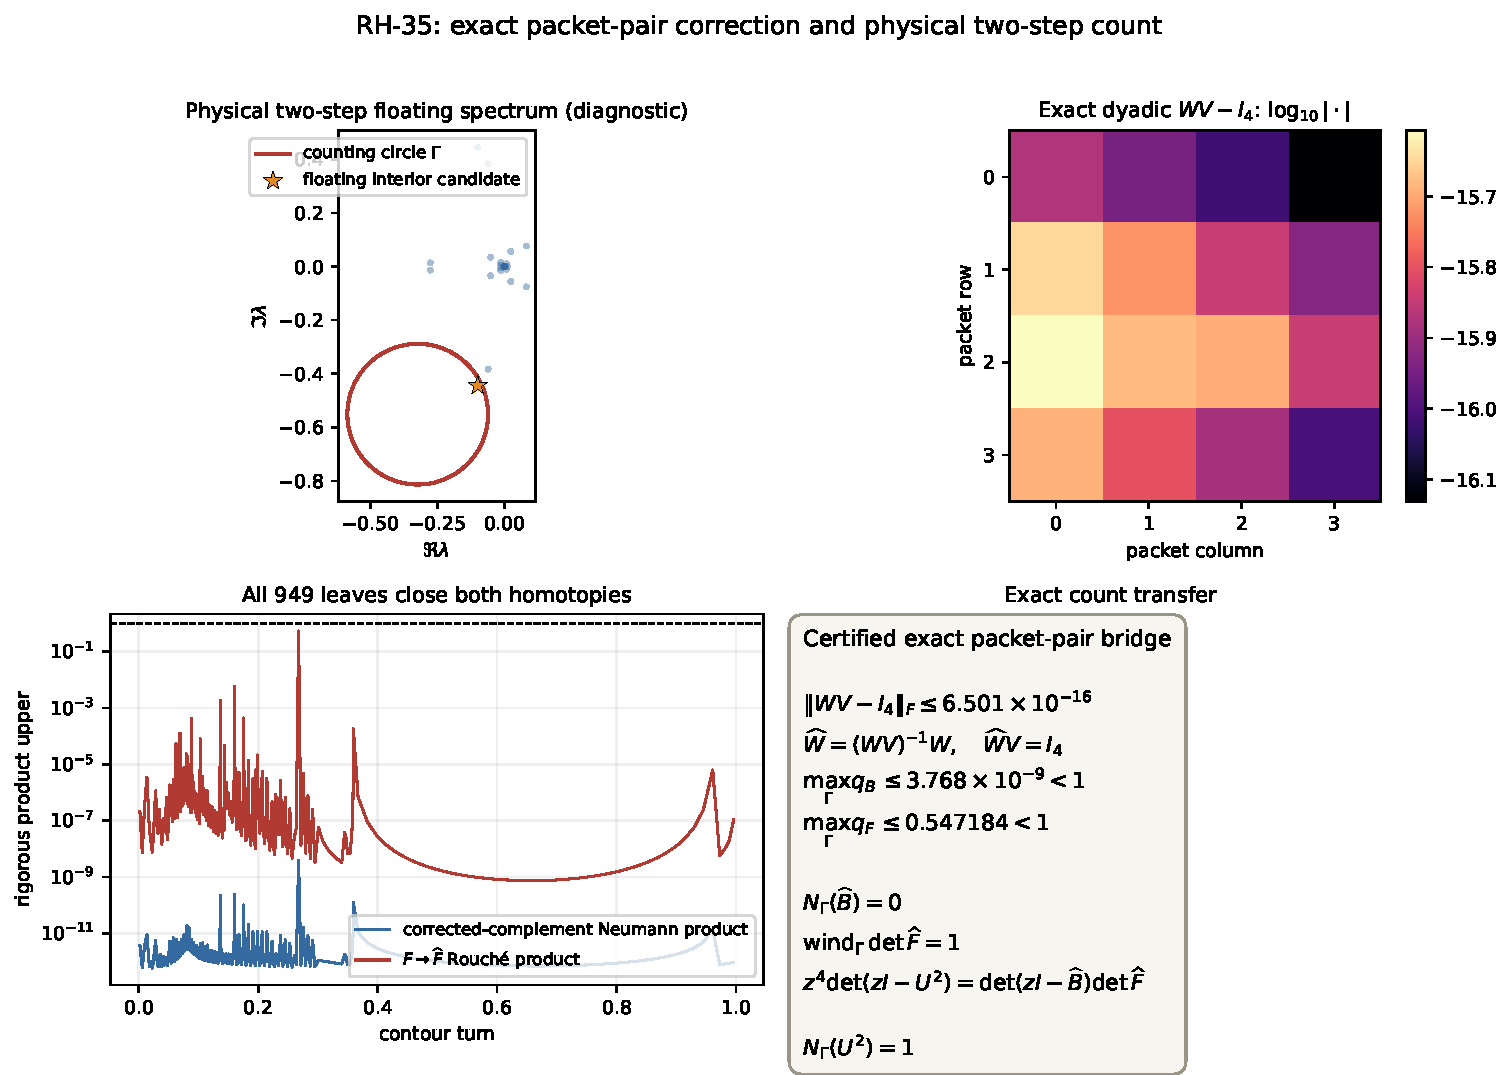
\includegraphics[width=\textwidth]{figures/packet_pair_physical_count.pdf}
\caption{Exact packet-pair transfer.  Top left: floating spectrum of the
physical two-step matrix, shown only as a diagnostic.  Top right: exact
dyadic entries of \(WV-\Id_4\).  Bottom left: all \(949\) rigorous
corrected-complement and Feshbach products.  Bottom right: the exact
coordinate and count ledger.}
\label{fig:physical-count}
\end{figure}

\section{Main physical count theorem}
\label{sec:main-theorem}

\begin{theorem}[Exact stored physical two-step count]
\label{thm:physical-count}
For the exact \(2048\times2048\) Perron/parity-extracted physical two-step
matrix
\[
 \Aphys=U^2
\]
defined by the stored binary64 factors at \(\sigma=10^{-2}\),
\begin{equation}
 N_\Gamma(\Aphys)=1.
 \label{eq:physical-count-one}
\end{equation}
Thus exactly one eigenvalue lies in the circle, counted algebraically.
\end{theorem}

\begin{proof}
\Cref{tab:leaf-results} verifies both gates in
\cref{thm:leafwise-transfer} on all \(949\) leaves.  Applying
\cref{eq:rh34-input,eq:transferred-counts} gives
\[
 N_\Gamma(\widehat B)=0,\qquad
 \wind_\Gamma\det\widehat F=1.
\]
The exact stored circle has center
\[
 -0.3233504401504541-0.5508412474453575i
\]
and radius \(0.2624987592858511\).  Exact dyadic arithmetic gives
\[
 |c|^2-r^2
 =
 \frac{
 27509112334457289433346968324839
 }{
 81129638414606681695789005144064
 }>0,
\]
so zero lies outside the disk and
\(\wind_\Gamma z^4=0\).  Taking the winding of
\cref{eq:corrected-schur-identity} yields
\[
 N_\Gamma(\Aphys)
 =N_\Gamma(\widehat B)
  +\wind_\Gamma\det\widehat F
 =0+1.
\]
\end{proof}

\begin{corollary}[Corrected physical Feshbach zero]
\label{cor:corrected-zero}
The corrected complement has no eigenvalue in the closed disk,
\(\widehat F\) is holomorphic there, and
\(\det\widehat F\) has exactly one zero in the disk, counted with
multiplicity.
\end{corollary}

\begin{proof}
The complement homotopy excludes boundary crossings and preserves the
RH-34 zero interior count.  Hence
\((z\Id-\widehat B)^{-1}\) is holomorphic in the disk.
The transferred winding is one, so the ordinary argument principle gives
the assertion.
\end{proof}

\begin{remark}[What the theorem now identifies]
\label{rem:what-identifies}
The count no longer belongs only to the \((n+m)\)-dimensional stored
augmented realization.  It belongs to the full \(n\)-dimensional matrix
\(\Aphys=U^2\) itself.  The theorem still concerns the exact finite
serialized discretization; the term \emph{physical} does not mean that a
continuum operator limit has been proved.
\end{remark}

\section{Audit trail and reproducibility}
\label{sec:audit}

The committed archive contains:

\begin{enumerate}
 \item the exact rational numerator and denominator of every entry of
       \(WV-\Id_4\);
 \item the exact-pair, block-majorant, leaf-extrema, count, timing, and hash
       fields in the main certificate JSON;
 \item all \(949\) leaf rows, including the projected inverse,
       computable RH-28 ratio, remainder coefficient, full inherited ratio,
       corrected complement product, corrected Feshbach difference, and
       both homotopy denominators;
 \item a floating spectrum pilot clearly labeled nonvalidated;
 \item dependency hashes for the RH-28 arc ledger, RH-33 resolvent atlas,
       RH-34 count theorem, physical model builder, and componentwise
       arithmetic; and
 \item eight unit and archive tests, including a synthetic proof of the
       \(\Aphys\oplus0_m\) coordinate identity.
\end{enumerate}

The rigorous certificate takes approximately \(8.0\) seconds on the
reported server.  The exact dyadic Gram stage takes under one second; the
dominant step is the blockwise componentwise enclosure of \(\Aphys Q\).
Timings are diagnostics.

The outward arithmetic assumes IEEE binary64 round-to-nearest operations,
conservative operation counts, no overflow, and no harmful underflow
\citep{Higham2002,Rump2010}.  Exact Gram products use rational integer
arithmetic, and the final positive scalar combinations use \(256\)-bit Arb
\citep{Johansson2017}.

\section{Scope, limitations, and next gates}
\label{sec:limitations}

The theorem closes the finite-coordinate bridge at one stored scale.  It
does not establish the following.

\begin{enumerate}
 \item The stored sparse matrix is not enclosed relative to the exact
       Gaussian integral kernel or an infinite-dimensional transfer
       operator.
 \item The count has not been continued through smaller noise scales and
       increasing dimensions.
 \item No interval enclosure of the physical eigenvalue location is given.
       The theorem is a contour count, not a validated eigenvalue box.
 \item The floating observation that most eigenvalues have tiny modulus is
       not an exact rank theorem.
 \item No self-adjoint generator, prime-power trace formula,
       \(T\log T\) counting law, zeta-zero identification,
       Hilbert--P\'olya construction, or implication for the Riemann
       hypothesis is obtained.
\end{enumerate}

The immediate stored-scale chain is now complete:
\[
\begin{gathered}
\text{projected winding}
\longrightarrow
\text{stored Feshbach winding}\\
\longrightarrow
\text{zero complement count}
\longrightarrow
\text{physical two-step count}.
\end{gathered}
\]

The next mathematically distinct gates are scale continuation and spectral
localization.  A natural continuation paper would combine:

\begin{enumerate}
 \item the exact packet correction at several smaller \(\sigma\);
 \item a compressed or sparse replacement for dense full-spectrum
       diagnostics;
 \item validated disks for the unique physical eigenvalue;
 \item perturbation bounds linking adjacent stored dimensions and noise
       scales.
\end{enumerate}

Only after such finite-scale continuation would a continuum or zero-noise
question become well posed.

\section{Conclusion}
\label{sec:conclusion}

The stored packet pair missed exact biorthogonality by approximately
\(6.5\times10^{-16}\).  That discrepancy is tiny, but the preceding papers
correctly refused to erase it algebraically.  Exact dyadic arithmetic now
shows that the packet Gram is invertible and supplies a canonical rational
dual correction.

The correction changes the complement block by at most
\(4.704\times10^{-15}\).  The inherited nonnormal resolvent atlas amplifies
this to a worst complement product of \(3.768\times10^{-9}\), still far
below one.  The more demanding Feshbach comparison retains the complete
primal--dual remainder and closes with product \(0.547185\).

Consequently the corrected packet/complement system has zero complement
count and winding one.  Exact coordinate factorization then transfers that
count to the full stored physical two-step matrix:
\[
 N_\Gamma(U^2)=1.
\]
This is the first point in the chain where the unique contour count belongs
to the physical \(2048\)-dimensional finite matrix rather than only to a
projected or augmented stored realization.  Extending it across scales
remains a separate problem.

\appendix

\section{Derivation of the block majorants}
\label{app:majorants}

From \(\Delta W=-G^{-1}HW\),
\[
 \norm{\Delta W}_2
 \leq \norm{G^{-1}}_2\norm H_2\norm W_2
 \leq \delta_W.
\]
Because \(\Delta Q=-V\Delta W\),
\(\norm{\Delta Q}_2\leq\delta_Q\).
The exact block differences are
\begin{align*}
 \widehat D-D
 &=\Delta W\Aphys V,\\
 \widehat C-C
 &=-V\Delta W\Aphys V,\\
 \widehat E-E
 &=\Delta W\Aphys Q
   -W\Aphys V\Delta W
   -\Delta W\Aphys V\Delta W,\\
 \widehat B-B
 &=-V\Delta W\Aphys Q
   -Q\Aphys V\Delta W
   +V\Delta W\Aphys V\Delta W.
\end{align*}
These identities explain why the certificate uses the directly enclosed
quantities
\[
 \Aphys V,\qquad \Aphys Q,\qquad D,\qquad C,\qquad E,
\]
instead of a crude global bound for \(\norm{\Aphys}\).

\section{Reproduction}
\label{app:reproduction}

From this paper directory, run
\begin{verbatim}
PYTHONDONTWRITEBYTECODE=1 python -m pytest -q -p no:cacheprovider
PYTHONDONTWRITEBYTECODE=1 python experiments/build_archive.py
MPLBACKEND=Agg python experiments/make_figures.py
python experiments/verify_archive.py
\end{verbatim}
The complete rigorous certificate is rebuilt by
\begin{verbatim}
OPENBLAS_NUM_THREADS=32 OMP_NUM_THREADS=32 \
PYTHONDONTWRITEBYTECODE=1 python \
  experiments/run_packet_pair_certificate.py \
  --sigma 0.01 --chunk-size 256
\end{verbatim}
The manuscript is compiled with
\begin{verbatim}
latexmk -pdf -interaction=nonstopmode -halt-on-error main.tex
\end{verbatim}

\bibliographystyle{plainnat}
\bibliography{references}

\end{document}
